\documentclass[crop=false,class=mitthesis,oneside,font=12pt]{standalone}
%----------------------------Preamble-------------------------------%
\usepackage{amsmath}
%\newcommand{\angstrom}{\textup{\AA}}
\usepackage{microtype}
\usepackage{graphicx}
\graphicspath{{./images/}}
%\usepackage{multirow}
\usepackage{rotating}
\usepackage{natbib}
\usepackage{url}
\usepackage{booktabs}
\usepackage{makecell}
\usepackage{graphicx, float}            % Graphics/Images.
\usepackage{pgfplots, tikz}             % Drawing/graphing tools.
\usetikzlibrary{
    calc,                   % Calculating right angles and more.
    angles,                 % Drawing angles within triangles.
    arrows.meta,            % Latex and Stealth arrows.
    quotes,                 % Adding labels to angles.
    positioning,            % Relative positioning of nodes.
    decorations.markings,   % Adding arrows in the middle of a line.
    patterns,
    arrows,
    shapes,
    shapes.geometric,
    cd,
    hobby,
    babel
}                                       % Libraries for tikz.
\pgfplotsset{compat=1.9}                % Version of pgfplots.
\usepackage[]{pdfpages}
% for line numbers comment the next two lines before final submission
\usepackage{lineno}
\linenumbers*[1]
% use fancyhdr, to enable page style stuff (below)
\usepackage{fancyhdr}
\setlength{\headheight}{15.2pt}
\renewcommand{\headrulewidth}{0pt}

\pagestyle{plain}
\usepackage{import}                     % Import external files.
\usepackage[subpreambles=false]{standalone}      % Complileable sub files.
\begin{document}
\chapter{Introduction}
% The upper atmosphere of the earth (90 km+, defined in section \ref{sec:str}) is influenced by forcing from below (the lower atmosphere) as well as forcing from above (the sun). The upper atmosphere is in a weak plasma state due to ionization of chemical species by high energy solar radiation. Understanding the processes in the upper atmosphere thus is important. In this thesis, we study the upper atmosphere during two phenomenon: one involving particle entry and the other involving dynamics generated by thermal changes.
The Ionosphere-Thermosphere (IT) system is the region of the Earth's upper atmosphere which is influenced by energy inputs from the sun and the lower atmosphere. The solar inputs are in the form of high energy Ultra Violet (UV) and X-ray radiation; and, the energetic solar particles that gives rise to observable phenomena such as the aurora. The inputs from the lower atmosphere are in the form of various waves and tides that alter the temperature and the composition of the IT system. The IT region has been studied for decades; however, owing to complex non-linear photochemical, electro-dynamical and collisional interactions involving the Earth's magnetic field, the ionospheric plasma, and the thermospheric neutral constituents, it is not completely understood. Understanding the processes in the IT system is important as many satellites, including the International Space Station (ISS) reside here. The compositional and dynamic changes the IT system introduced by sudden deviation in energy inputs (especially solar inputs) could affect our communication systems and expose astronauts to hazardous radiation environments. In addition, studying the Earth's IT system would also act as a starting point in understanding the upper atmosphere of other planets. In this thesis, study of the IT system's response to two different process is conducted; one involving particle entry and the other involving dynamics generated by thermal changes.

\section{Dissertation Outline}

This thesis is focused on observing the IT system using a ground-based multi-spectral imager known as High Throughput \& Multi Slit Imaging Spectrometer (HiT\&MIS). Based on observations, questions on two different phenomena are studied and answered. The first phenomenon involves estimation of the energetics of solar particle entry during an auroral event by multi-spectral measurements. Specifically, the feasibility of using multi-spectral measurement of auroral brightnesses to simultaneously derive energy and flux of the precipitating auroral electrons is addressed. The second phenomenon involves temperature and composition changes in the polar upper atmosphere due to the effects of total solar eclipse and geomagnetic disturbances that lead to atmospheric waves propagating towards the equator. 

In this first chapter, a simplified theoretical background on a planetary atmosphere, the Earth's upper atmosphere and the IT system is given. Also included is information on how the HiT\&MIS observations are tied to the above mentioned phenomena in the IT system. In chapter 2, details on different instruments that were used for this thesis are provided with emphasis on HiT$\&$MIS. Chapter 3 describes how multi-spectral imaging was used to simultaneously derive the energy and flux during an auroral event. Chapter 4 presents the characterization of Traveling Ionospheric Disturbances (TIDs) generated by Atmospheric Gravity Wave (AGWs) observed using multiple instruments. In Chapter 5, conclusions on the thesis questions mentioned in Section \ref{thesis_q}, based on results obtained in Chapter 3 and 4 are provided.

This dissertation contains modified versions of the publications "Derivation of the energy and flux morphology in an aurora observed at mid‐latitude using multi‐spectral imaging"  by \citet{aryal_energy} (Chapter 3) and "Multi-spectral and multi-instrument observation of TIDs following the Total Solar Eclipse of August 21, 2017" by Aryal et al. (submitted, Chapter 4).

 \section{Theory of the Planetary Atmosphere}
% \begin{figure}[htp]
% 	\centering\includegraphics[width=32pc]{planetary_atmos.png}
% 	\caption{Simplified planetary atmosphere in one dimensional plane-parallel geometry.}
% 	\label{fig:atmos}
% \end{figure}
  \begin{figure}[H]
            \centering
            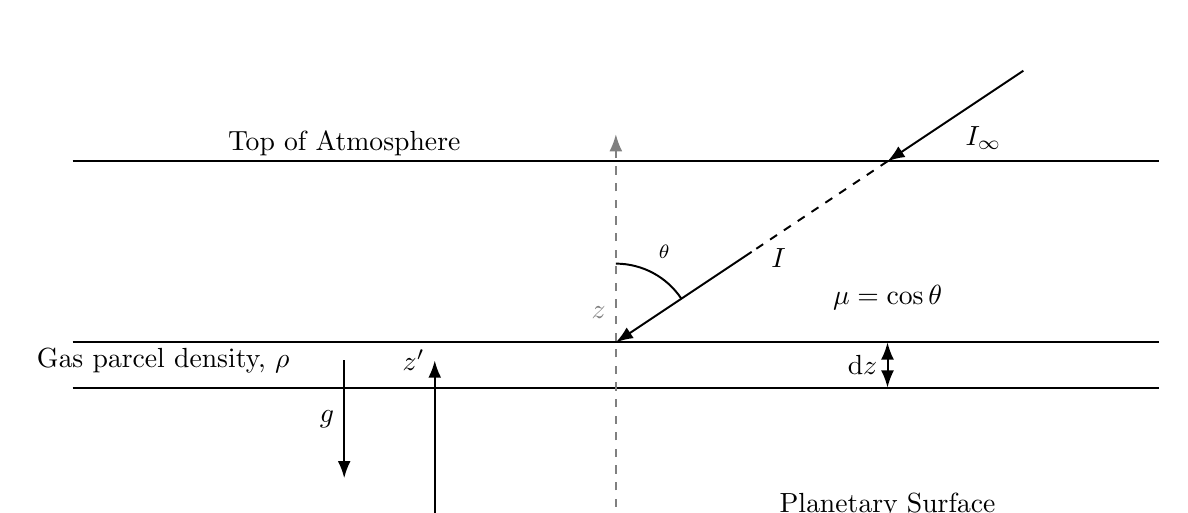
\begin{tikzpicture}[>=Latex, line width=0.25mm,scale=1.15]
                \coordinate (O) at (0,0) {};
                \coordinate (Q) at (0,2) {};
                \coordinate (P) at (3,2) {};
                \draw (-6,-2) to (6,-2);
                \draw (-6,-0.5) to (6,-0.5);
                \draw (-6,0) to (6, 0);
                \draw (-6,2) to (6, 2);
                \draw[dashed] (3,2) to 
                    node [below left=4mm and 3mm] {$I$} (1.5, 1);
                \draw[->] (1.5,1) to (0,0);
                \draw[dashed, ->, gray] (0,-2)
                    to node [above left] {$z$} (0,2.3);
                \draw[->] (4.5,3) to node [below right] {$I_{\infty}$} (3,2);
                \draw[<->] (3,-0.5) to node [left] {$\textrm{d}z$} (3,0);
                \draw[->] (-3, -0.2) to node [left] {$g$} (-3, -1.5);
                \draw[->] (-2, -2) to (-2, -0.2) node [left] {$z'$};
                \node at (-3, 2.2) {Top of Atmosphere};
                \node at (-5, -0.2) {Gas parcel density, {$\rho$}};
                \node at (3, -1.8) {Planetary Surface};
                \node at (3, 0.5) {$\mu= \cos\theta$};
                \pic[%
                    "\scriptsize{$\theta$}",
                    angle eccentricity=1.3,
                    angle radius=1.0cm,
                    -,
                    draw=black
                ]   {angle=P--O--Q};
            \end{tikzpicture}
            \caption{Simplified planetary atmosphere in one dimensional plane-parallel geometry.}
         	\label{fig:atmos}
        \end{figure}
        
This section follows \citet{chamberlain1990theory}, \cite{rees1989physics}, etc. to provide a simplified background on the theory of the planetary atmosphere. Assuming 1D plane-parallel geometry (Figure \ref{fig:atmos}) the pressure (p) gradient on a small parcel of gas with density ($\rho$) contained in small height (dz) of a planet with gravity (g) can be written as:
\begin{equation}
\label{eq:he}
\large
\frac{dp}{dz} = -g(z) \rho.
\end{equation}
This comes from applying Newton's second law to the parcel of gas. Assuming that the gas parcel follows the ideal gas law, the pressure ($p$) can be written as $\rm \frac{\rho}{M} k_B T$, where $k_B$ is the Boltzmann's constant, $T$ is the temperature, and $M$ is the molecular mass of the gas. Replacing the pressure and assuming both the pressure and the temperature to remain constant at all altitude ($z$), equation \ref{eq:he} becomes:
\begin{equation*}
\large
\frac{dp}{dz}= -p \frac{M g}{k_B T} = -\frac{p}{H}  \\
\end{equation*}
\begin{equation*}
\large
\implies \frac{dp}{p}=-\frac{dz}{H}
\end{equation*}
\begin{equation}
\label{eq:p}
\large
\implies p (z)= p(z_{0}) e^{-\frac{z-z_{0}}{H}} \implies n(z)= n(z_{0}) e^{-\frac{z-z_{0}}{H}} ,
\end{equation}
where, H = $\rm \frac{k_B T}{M g}$ is known as the scale height, $z_0$ is the reference altitude and n is the number density. The scale height $H$, is the height at which the pressure (and the number density) drops by $\rm \frac{1}{e}$. For a well-mixed atmosphere, $M$ is the mean molecular weight of all the atmospheric gases. The chemical species diffusively separate for an unmixed atmosphere and each chemical species follow their own scale height $H_j$= $\rm \frac{k_B T}{M_{j} g}$. Here,  $H_j$ and $M_j$ are the scale height and the molecular mass of the j$^{\rm th}$ atmospheric species, respectively.

So far it is assumed that the temperature and the gravity are constant with respect to the atmospheric height. This is an ideal over-simplification as the gravity drops smoothly with height and the temperature changes differently at different layers of the atmosphere (see Section \ref{sec:str}) depending on various inputs into the atmosphere. There are also different chemical and physical processes that transport atmospheric constituents and break hydrostatic equilibrium. Thus, in general, planetary atmospheres are sliced into thin layers where ideal conditions are assumed to hold. 

The column density, N, is defined as the density integrated along a column above a vertical height (z), i.e:
\begin{equation}
\label{eq:N}
\large
N(z) = \int_{z}^{\infty} n(z')~dz'
\end{equation}
Now, using equations \ref{eq:p} and \ref{eq:N}, N becomes:
\begin{equation}
\label{eq:colden}
\large
N(z) =\int_{z}^{\infty} n(z_{0}) e^{-\frac{z'-z_{0}}{H}} dz' \implies N(z) =H n(z),
\end{equation}
which gives an estimation of the scale height in terms of the column density.


\subsection{Radiative Energy Deposition}
\label{sec:edep}
Energy deposition in the atmosphere is mainly governed by two processes involving radiation -- absorption and ionization. The cross-sections of absorption ($\sigma_a$) and ionization ($\sigma$) control where the energy is deposited and are functions of the wavelength of incident radiation. In a plane-parallel atmosphere, for a single chemical species, $j$, with number density $n_j$, that gets illuminated with solar radiation of intensity $I$, the ionization rate $q_j$, is given by the product of the radiation intensity, the ionization cross-section, and the density of the chemical species $j$. In mathematical form, the total ionization rate $q$, is given by:
\begin{equation}
\label{eq:ino}
\large
q(\lambda,~z) = \sum_{j}~I({\lambda},~z)~\sigma_{j}(~\lambda)~n_{j}(z)
\end{equation}
According to Beer's law, the irradiance at height z, considering a single species j, is given by: 
\begin{equation}
\label{eq:beer}
\large
I(\lambda,~z) = I_{\infty}~(\lambda)~e^{-\tau_{j}(\lambda,~z)},
\end{equation}
where I$_\infty$ ($\lambda$) is the irradiance on top of the planetary atmosphere and $\tau_j$ is the optical depth of a single species j. The total optical depth is given by:
\begin{equation}
\label{eq:taua}
\large
\tau(\lambda,~z)~= \sum_{j}~\sigma_{aj}(\lambda)~\int_{z}^{\infty}~n_{j}(z')~dz',
\end{equation}
where $\sigma_{aj}$($\lambda$) is the absorption cross section for the species j. From equations \ref{eq:colden} and \ref{eq:taua}, and considering off-zenith geometry (see Figure \ref{fig:atmos}) with solar zenith angle $\theta$, and defining $\mu$ = cos$~\theta$, the following is obtained: 
\begin{equation}
\label{eq:tau}
\large
\tau(\lambda,~z)~= \sum_{j}\frac{~\sigma_{aj}(\lambda)~N_{j}(z)}{\mu} =~\sum_{j}\frac{~\sigma_{aj}(\lambda)~n_{0j}~H_{j}~e^{-(\frac{z-z_{0}}{H_{j}})}}{\mu}.
\end{equation}
Combining equations \ref{eq:beer} and \ref{eq:tau}, the irradiance at a height z is:
\begin{equation}
\label{eq:irr}
\large
I(\lambda,~z) = I_{\infty}~(\lambda)~ e^{~\sum_{j}\frac{~\sigma_{aj}(\lambda)~n_{0j}~H_{j}~e^{-(\frac{z-z_{0}}{H_{j}})}}{\mu}}.
\end{equation}

\subsection{The Chapman Function}
\begin{figure}[H]
	\centering\includegraphics[width=35pc]{chapman_slm.png}
	\caption{A typical Chapman function in the Earth's atmosphere due to 30 nm solar radiation at various solar zenith angles. Source: \cite{stan_lec1}.}
	\label{fig:chapman}
\end{figure}

Considering only a single atmospheric species j, and radiation incident in the nadir direction ($\theta$ = 0 in Figure \ref{fig:atmos}), using equation \ref{eq:ino} and \ref{eq:irr} the ionization rate is obtained as:
\begin{equation*}
\large
q_{j}(\lambda,~z)=~I_{\infty}~e^{-\tau_{j}~(\lambda,~z)}~\sigma_{j}~n_{0j}~e^{-\frac{z-z_{0}}{H_{j}}}
\end{equation*}
\begin{equation}
\label{eq:chp}
\implies \large
q_{j}(\lambda,~z)=~I_{\infty}~\sigma_{j}~n_{0j}~e^{\big (-\frac{z-z_{0}}{H_{j}}-\tau_{j}~(\lambda,~z) \big )}.
\end{equation}
Equation \ref{eq:chp} is known as the Chapman function for a single species j. Figure \ref{fig:chapman} shows profiles of typical Chapman functions due to 30 nm solar radiation at various solar zenith angles ($\theta$) for a single species. Notice that the ionization peaks around 150 km altitude in this case. Taking derivative of Equation \theequation ~with respect to height and setting it to 0 to optimize, i.e:
\begin{equation*}
\large{
\frac{d q_{j}(\lambda,~z)}{dz}=~ \frac{d[I_{\infty}~\sigma_{ij}~n_{0j}~e^{\big (-\frac{z-z_{0}}{H_{j}}-\tau_{j}~(\lambda,~z) \big )}]}{dz}=~0}
\end{equation*}
\begin{equation*}
\implies \large{
\frac{d q_{j}(\lambda,~z)}{dz}=~ I_{\infty}~\sigma_{ij}~n_{0j}~\Big [\frac{1}{H_{j}} + \frac{\tau_{j}(\lambda,~z)}{H_j}\Big ]~e^{(-\frac{z-z_{0}}{H_{j}}-\tau_{j}~(\lambda,~z))}}{dz}~=0
\end{equation*}
\begin{equation}
\implies \large{
\frac{1}{H_{j}} + \frac{\tau_{j}(\lambda,~z)}{H_j}}~=0 \implies \tau_{j}(\lambda,~z) =1,
\end{equation}
it is found the Chapman function is at $\tau_{j}$($\lambda$, z) =1 for the species j. Thus, the altitude at which $\tau_{j}$($\lambda$, z) =1 is where most of the energy is deposited for a particular species j at a particular wavelength. In an atmosphere with multiple species and the full spectrum of stellar radiation, there can be multiple Chapman peaks, giving rise to Chapman layers.

\section{Earth's Atmosphere}
\subsection{Structure of the Atmosphere}
\label{sec:str}
\begin{figure}[H]
	\centering\includegraphics[width=32pc]{vert_stu.jpg}
	\caption{Vertical structure of the Earth's atmosphere in terms of temperature, density of chemical species and where solar radiation at different wavelengths gets absorbed. Source: \cite{jemrt}.}
	\label{fig:vert_str}
\end{figure}

The Earth's atmosphere is stratified into many different layers (Figure \ref{fig:vert_str}) based on the neutral temperature profile (Figure \ref{TI_temp_var}), how the chemical species mix (Figure \ref{fig:neu_den}) and the differences in dominant physical processes, etc. In terms of the neutral temperature profile, the Earth's atmosphere is divided into the following:
\begin{itemize}
	\item the troposphere (0--15~km in altitude) is where temperature decreases with altitude due to decrease in infrared radiation from the Earth. This is the layer where most of the terrestrial weather occurs. Molecular species (especially N$_2$ and O$_2$) are dominant in the troposphere and all the gases are well-mixed.
	\item The stratosphere (15--50~km) is where there is an increase in temperature when compared to the troposphere as UV radiation gets absorbed by ozone (O$_3$), which is the dominant chemical species. Since the temperature increases with altitude, the stratosphere is thermodynamically stable.
\item  The mesosphere (50--90~km) is where the temperature decreases due to radiative cooling by CO$_2$ and NO. Balloons cannot reach above 40 km because of thinning air and satellites cannot reside here because atmoshpheric drag and gravity are too high compared to the upper atmosphere. Thus, in-situ measurements of the mesosphere is not possible and makes it more difficult to study compared to the other layers.
	\item The thermosphere (90--600~km) is where the temperature increases rapidly due to absorption of high energy solar radiation (UV and X-rays) and lack of cooling mechanism. The number density in the thermosphere is orders of magnitude lower than in the troposphere, and the atomic species start to dominate as molecules are dissociated by solar radiation. High energy solar radiation also ionizes chemical (neutral) species in the thermosphere creating the ionosphere.  Optical emissions (like airglow and aurora) occur in this region of the atmosphere generated by various photochemical and plasma processes.
\item  The exosphere (1000+~km) is marked by extremely low density gas that leak from the Earth's atmosphere. There is no upper boundary of the exosphere as it merges with interplanetary space. The exosphere is sometimes not considered part of the Earth's atmosphere as the conditions are more like space. The lighter gas (mostly hydrogen and helium) in this layer are leaking out into space.
\end{itemize}
\begin{figure}[H]
	\centering\includegraphics[width=35pc]{okl_temp_stru_slr_min_max.png}
	\caption{Temperature structure of the Earth's atmosphere based on MSIS \citep{msie}. Notice sharp rise in temperature in the transition region between the Mesosphere and the Thermosphere after which the temperature plateaus. Source: \cite{stan_lec1} }
	\label{fig:TI_temp_var}
\end{figure}

In terms of mixing, the Earth’s atmosphere is divided into two regions (Figure \ref{fig:neu_den}). 
\begin{itemize}
	\item The heterosphere (up to 100 km) is where all the chemical species are well-mixed due to turbulence. It is dominated by heavier molecules like O$_2$ and N$_2$. 
	\item The homosphere ($>$ 100 km) is where chemical species are not well-mixed due to diffusion and the density structure of each species is determined by mass. That is, the lighter chemical species are found higher in the atmosphere. Thus, the lighter atoms (like O) start being the dominant chemical species. 
\end{itemize}
\begin{figure}[H]
	\centering\includegraphics[width=35pc]{ok_dens_str_neu.png}
	\caption{Neutral density structure of the Earth's atmosphere. In the fully mixed lower atmosphere, the neutral species density have the same scale height, for the unmixed upper atmosphere each species different scale heights and start seperating. Source: \cite{stan_lec1}}
	\label{fig:neu_den}
\end{figure}

In terms of differences in dominant physical processes, the Earth's atmosphere is divided into: 
\begin{itemize}
	\item the lower atmosphere (0-15 km), which is dominated by turbulence and decrease in temperature with increasing heights. 
	\item The middle atmosphere (15-90 km) which is dominated by turbulence and neutral dynamics, but can also effected by very high energy (1 MeV+) solar particles.
	\item The upper atmosphere (90 km and above) which is the focus of this thesis. High energy solar radiation (UV and X-rays) and plasma processes dominate this region. However, it is also influenced by the lower atmospheric tides and waves. 
\end{itemize}
Since the upper atmosphere and specifically the IT system is the focus of this thesis, the rest of the description provided in this chapter is on the upper atmosphere.

%%%%
\subsection{Upper Atmosphere}

The upper atmosphere (90 km+) is the first to receive the direct solar radiative energy input (dominant in mid and low latitudes) as well as the solar charged particle input (dominant in higher latitudes) via the magnetosphere. Most of the high energy solar radiation is deposited in the upper atmosphere as the height where the total optical depth, $\tau$ =1 ($\tau$ as defined in equation \ref{eq:taua}) for these wavelengths lie there (Figure \ref {fig:tau1}).  The high energy solar radiation (X-rays and UV) also ionize the neutral constituents present in the upper atmosphere, creating the ionosphere, the ionized part of the upper atmosphere (Figure \ref{fig:iono_layer}). Thus, the upper atmosphere is a mixture of neutral, ions and electrons whose interactions are then affected by the presence of the Earth’s magnetic field. This thesis is focused on the remote sensing of the one specific part of the upper-atmosphere, i.e., the ionosphere and the thermosphere, sometimes regarded as one system and referred to as the IT system.
\begin{figure}[H]
	\centering\includegraphics[width=32pc]{ionosphere_layers.jpg}
	\caption{Different layers of the ionosphere during the day and during night. Source:  Encyclopedia Britannica, Inc.}
	\label{fig:iono_layer}
\end{figure}

\begin{figure}[H]
	\centering\includegraphics[width=35pc]{tau1.png}
	\caption{Heights where the total optical depth, $\tau$ =1, as a function of wavelength.  $\tau$ =1 is where the the maximum absorption of solar radiation occurs. Also shown are the major chemical responsible for the absorbtion. Source: \cite{thomas2002radiative}. }
	\label{fig:tau1}
\end{figure}

\subsubsection{Thermosphere}
\label{therm}
 Thermosphere is the region in the upper-atmosphere of the Earth's ($\sim$ 90-600 km) where the neutral gas density is orders of magnitude lower compared to the sea level (Figure \ref{fig:neu_den}) and the temperature is high (around 1500 K) due to heating from high energy solar radiation and lack of cooling mechanism. The boundary between the mesosphere and the thermosphere is characterized by rapid increase in temperature with increasing altitude (Figure \ref{fig:TI_temp_var}). The low density environment decreases collisional interaction between the atmospheric constituents, and they start diffusing separately unlike in the lower atmosphere. The lighter atomic constituents (for example Oxygen atom, O), which are almost absent in the lower atmosphere when compared to the molecular (for example, Nitrogen, N$_2$ and Oxygen, O$_2$ molecules), become the dominant chemical species (Figure \ref{fig:neu_den}). The reason behind this is two fold- the molecular diffusion time-scale for heavier molecules (like N$_2$ and O$_2$) is faster than the lighter atoms (like O), and the increase in high energy solar radiation in the thermosphere dissociate molecules into lighter atoms. 

% Thermosphere is also where most of the Low Earth Orbit (LEO) satellites, including the International Space Station (ISS) reside. So, studying the thermosphere (and the embeded ionosphere) also helps in quantifying the effects of upper-atmospheric weather (referred as Space Weather hereafter) on expensive satellites as well as health effects on Astronauts. In addition, radio technologies based on satellites (GPS, satellite internet, etc.) could get disrupted by Space Weather. Like terrestrial weather, the long term goal for Space Weather studies is to predict adverse weather before-hand to limit economic damage caused by such events.
%%%%temperature structure plot

%%%Solar spectrum


%%%%%% Absorbtion of solar radiation
% \begin{figure}[H]
% 	\centering\includegraphics[width=35pc]{slr_rd_abs.png}
% 	\caption{Solar energy deposition in the Earth's atmosphere. Notice that most the highest energy radiation (< 200 nm) are absorbed before thy reach 100 km. Plot courtesy of Dr. Stan Solomon, NCAR }
% 	\label{fig:sl_rad_abs}
% \end{figure}

\begin{figure}[H]
	\centering\includegraphics[width=35pc]{thm_dens.png}
	\caption{Density structure of neutral and ionic species in the Earth's atmosphere based on MSIS and IRI climatological models. Notice lighter atoms and ions are only present above $\rm \sim$ 100 km. Source: \cite{stan_lec2}.}
	\label{fig:TI_dens}
\end{figure}

\subsubsection{Ionosphere}
Ionization due to high energy solar radiation plus collisional ionization by energetic particles of the upper atmospheric neutral constituents creates a weakly ionized region known as the ionosphere (about 60-1000 km). Ionosphere, therefore, is the extension of the thermosphere (and upper mesosphere), i.e, the part of the thermosphere that gets ionized by the solar radiation. During the daytime, when the ionizing source (sun's high energy radiation) is incident on the ionosphere, it gets stratified into different layers and extends into the mesosphere. During the night time, the electrons and ions recombine and the plasma density decreases orders of magnitudes but do not go away completely.

\subsubsection{Ionospheric Layers}
Different part of the high energy solar radiation (daytime) ionize different neutral species which leads to ion density peaking at few specific heights making the ionosphere vertically stratified. As discussed in Section \ref{sec:edep}, peak energy at a particular wavelength and for a species is deposited at the altitude where the optical depth, $\tau$ = 1 (Figure \ref{fig:tau1}). Since the full solar (or stellar spectrum) is incident on all of the chemical elements, the total $\tau$ = 1 altitude for all wavelength peaks at different altitudes causing energies to be deposited at peaks altitudes creating Chapman layers. This stratification ionization peaks giving rise to the ionospheric layers. During the night some of the stratified layers vanish due to recombination and absence of an ionizing source (Figure \ref{fig:iono_layer}). The different layers of the ionosphere are:
\begin{itemize}
\item the D-layer is only present during the daytime and extends from the upper mesosphere to the lower thermosphere (around 60-90 km).
\item The E-layer was the first ionospheric layer discovered, and hence was named the Electric-later (or the E-layer). The other layers above and below the E-layer were named going up or down the alphabet (the D-layer is below the E-layer for example). It ranges from around 90 km to 150 km in altitude.
\item F-layer, is the topmost layer of the ionosphere and splits into two layers, F1 and F2, during the daytime. During the night time, the two layers merge into a single F-layer. The altitude range of the F range is from around 150 km to 1000 km.
\end{itemize}

\section{Magnetosphere} 
\label{magne}
The continuous stream of charged particles from the Sun (solar wind) with its embedded magnetic field, known as the Interplanetary Magnetic Field (IMF), hits the Earth and pushes and distorts the Earth's magnetic field. This creates a long cigar-shaped region where charged particle motion is controlled by Earth's magnetic field region, called the magnetosphere, that is connected to the IMF at its edges (see Figure \ref{fig:magnetosphere}). 
\begin{figure}[htp]
	\centering\includegraphics[width=32pc]{magneto.jpg}
	\caption{Magnetosphere of the Earth and associated current systems. Source: \citet{pollock2003role} }
	\label{fig:magnetosphere}
\end{figure}

To understand the magnetosphere, a brief description of basic plasma physics is required. The Lorentz force ($\bf{F}$) on a collection of charge particles with total charge q, moving at a velocity $\bf{v}$, in a magnetic ($\bf{B}$) and a electric field ($\bf{E}$) is given by:
\begin{equation}
\label{eq:lorentz}
{\bf F}~=~\rm q~({\bf E}+~{\bf v}\times{\bf B})
\implies m~\dot{\bf v}~=~\rm q~({\bf E}+~{\bf v}\times{\bf B}).
\end{equation}
From the equation \theequation, it follows that a single charged particle, in absence of a electric field, will gyrate around and drift along a constant magnetic field line (the guiding center) in a helical trajectory with a frequency of $\omega_{c}$ = $\frac{\rm q B}{m}$ , where m is the mass of the charge particle and B is the magnitude of the magnetic field. While the electrons and ions (positive) gyrate in opposite directions, they both drift along the magnetic field in the same direction (see Figure \ref{fig:drift}), this is what gives rise to the Field Aligned Current (FAC). The gyro-radius can then be expressed as: $r_L$= $\frac{v_\perp}{\omega_c}$=$\frac{m~v_\perp}{\rm q~B}$ ; where $v_\perp$ is the velocity perpendicular to guiding center. In addition to gyration, charged particles in the magnetosphere experiences different drift motions (see Figure \ref{fig:drift}). This is not just due to the geometry of the Earth's magnetosphere, but also due to difference in charge and mobility between electrons (negative charge, lighter) and ions (positive charge, heavier) that set up electric fields and currents in the magnetosphere. Some of these magnetospheric current system (like FAC) flow through the IT system.
\begin{figure}[H]
	\centering\includegraphics[width=25pc]{guiding_cntr_drft.jpg}
	\caption{Examples of drift motions that plasma's can undergo in presence of electric and magnetic fields. }
	\label{fig:drift}
\end{figure}

Gyrating charged particle around a magnetic field line have a magnetic moment, $\mu$ = ${I~A}$ , where, I is the average current due to gyration and A is the current's circular area, and so:
 \begin{equation}
 \mu~=~\frac{m~v^2_{\perp}}{2~B},
 \end{equation}which is a magnetic invariant if the magnetic field is changing slowly with time. In such case, the perpendicular energy of the particle, W$_\perp$ = $\frac{m~v^2_{\perp}}{2}$ is proportional to the magnetic field $\bf{B}$. When the particle moves in the region of stronger magnetic field, $v_\perp$ increases to keep $\mu$ invariant and the drift velocity along the guiding center (magnetic field line) $v_\parallel$, has to decrease due to conservation of energy. By defining, cos$~\alpha$ =$\frac{{\bf v\cdot B}}{v~B}$; where $\alpha$ is known as the pitch angle, the angle between the particle's velocity and the magnetic field.  When the pitch angle reaches 90$^\circ$, the particle gets reflected and this phenomenon is known as magnetic mirroring. Because of the Earth's magnetic field geometry, only particles with mirror points deep into the earth atmosphere can be lost into upper atmosphere, within an area known as the loss cone. These particles that get lost into the Earth's upper atmosphere give rise to auroras. In some region of the magnetosphere magnetic mirroring causes particles to get trapped within regions known as Van-Allen radiation belts. As electrons and protons have different mass (and hence different kinetic energy), there are two Van-Allen belts.
 
Electrical attraction between heavier ions and lighter electrons causes the plasma to re-distributes such that they behave like neutrals by canceling out charges beyond a certain distance. This screen out external electric fields over a characteristic distance known as the Debye length, $\lambda_d$ = $\sqrt{\frac{\epsilon_0~k_{B}~T_{e}}{n~e^2}}$; where $\epsilon_0$ is the electrical permittvity, k$_B$ is the Boltzmann's constant, T$_e$ is the electron temperature n is the electron number density.  In the Earth's ionosphere, the plasma is assumed to be nearly quasi-neutral (equal number of positive and negative charges) and in such case the Debye length is a measure of the distance scale over which positive and negative species act separately.

Plasmas in the Earth's upper atmosphere follow the Maxwell's equation in presence of both magnetic and electric fields:

\begin{equation}
\nabla\cdot \bf{E}~=~\frac{\rho_e}{\epsilon_0}
\end{equation}
\begin{equation}
\nabla \times {\bf E}~= -~\frac{\partial {\bf B}}{\partial t}
\end{equation}

\begin{equation}
\nabla\cdot \bf{B}~=~0
\end{equation}
\begin{equation}
\nabla \times B~=~\mu_{0}{\bf J}+\frac{1}{c^2}\frac{\partial \bf{E}}{\partial t},
\end{equation}
as well as the continuity equation,
\begin{equation}
\label{conti}
\frac{\partial n_{j}}{\partial t}+\nabla\cdot(n_{j}{\bf u}_{j})= P_j-L_j
\end{equation}

and the Ohm's law, ${\bf J}=\sigma {\bf E}$, where $\bf J$ is the current density, $\sigma$ is the conductivity tensor, and $\mu_0$ is the permeability of free space. $P_j$, $L_j$, $n_j$ and ${\bf u}_j$ are the production rate, loss rate, number density and velocity of species j. In the ionosphere, the production and loss rates are also coupled with the neutrals via ionization and recombination, respectively. 
\section{Ionosphere-Thermosphere (IT) system}
The thermosphere together with the charged portion of the upper atmosphere, i.e. the ionosphere, are coupled together via collision and production and loss processes. Thus, this coupled part of the upper atmosphere is known as the Ionosphere-Thermosphere (IT) system. In the lower portions of the IT, the density of the neural species are high enough to get affected by the neutral dynamics (weather) at lower altitudes. Hence, the IT system is influenced by forcing from above (sun) and below (tropospheric weather). Thus making it an ideal laboratory to study the solar-terrestrial interaction.
%\subsection{Why is IT hot ?}%I dont think you need to make a subsection out of it... just another paragraph will probably suffice. Sunip.

As mentioned in Section \ref{therm}, the thermosphere is characterized by rapid increase in temperature at its lower boundary. The ionization processes that create the ionosphere also creates an abundance of free energetic (hot) electron and ions which in-turn heat the neutral species (Figure \ref{fig:therm_heat}) collisionally. Auroral particle precipitation which occur generally in the higher latitudes also have similar heating effect. Such event cause frictional heating known as Joule heating due to enhancement of ionospheric currents.  In addition, various photochemical reaction in the thermosphere contribute in heating the ions and neutrals. Most of the cooling in the atmosphere occurs via radiation, which is dominated by radiation from CO$_2$ and NO. However, in the thermosphere the density of CO$_2$ and NO is orders of magnitude lower compared to the lower atmosphere and so the cooling rate is slow and thus the thermosphere remains hot. 
\begin{figure}[H]
	\centering\includegraphics[width=32pc]{thrm_heat.png}
	\caption{Overview of the thermospheric heating processes. Source: Dr. Stan Solomon, NCAR/UCAR.}
	\label{fig:therm_heat}
\end{figure}


\section{Magnetosphere-IT (MIT) system}
As discussed in Section \ref{magne}, the IT system cannot be de-coupled from the magnetosphere as the the Earth's magnetic field interacts with the ionosphere and vice versa. Their specific interaction is dictated by the geometry of the magnetic field lines at ionospheric heights. Around the magnetic equator, at ionospheric heights, the Earth's magnetic fields are nearly parallel to the surface of the Earth; while near the poles, they are nearly perpendicular. The interaction of plasma with the magnetosphere in conjunction with the co-rotation of the Earth also gives rise to various magnetospheric and ionospheric current system.  In addition, ejection or enhancement of earth-bound solar plasma due to magnetic activities on the sun can also cause changes to the Earth's magnetospheric structure. Furthermore, solar flares, which are sometimes related to plasma ejection events on the sun, can suddenly increase ionization causing perturbations in the magnetic fields at ionospheric heights. Additionally, various magneto-sonic waves, which effect the ionospheric plasma, can also disturb the IT system. In general, these coupling are non-linear in nature and can cause long term (days) Space Weather events that changes the properties of not only the ionosphere but also the thermosphere.

\subsection{MIT coupling}
To study the effect of MIT coupling, two examples are provided below. In the polar region of the Earth, the orientation of the magnetic field lines are almost perpendicular to the Earth's surface and carry the Field Aligned Currents (FACs) with them into and out of the ionosphere (Figure \ref{fig:mit_cpl_p}). The FACs are the manifestation of plasma gyration and magnetic mirroring drift as discussed in Section \ref{magne}. The FACs can also be enhanced by energetic plasma particles that get accelerated into the upper atmosphere via the magnetic field lines during magnetic re-connection events. The plasma carried by the FAC that are in the loss cone get lost into the ionosphere give rise to auroras and deposit energy. For the current system to close, the currents brought by the FACs diverge as they flow through the ionosphere and give rise to the Pedersen and Hall currents (Figure \ref{fig:mit_cpl_p}). Each of the associated currents have their characteristic conductivities ($\sigma_P$, Pedersen and $\sigma_H$, Hall conductivity). In the ionosphere these conductivities determine the exact interaction between the Pedersen and Hall currents. Figure \ref{fig:ped_hall} shows different physical regime encountered by FAC at different ionospheric layers. Any perturbation to the magnetic field disturbs these currents and ultimately the IT system, but the exact change depends on the nature of the magnetic disturbance.

\begin{figure}[H]
	\centering\includegraphics[width=35pc]{mit_cpl_i.png}
	\caption{Summary of how the Magnetosphere is coupled to the IT system at higher latitudes. Plasma flows (Field Aligned Current) via the magnetec field into and out of the ionosphere (Pedersen Currents) produces hall currents. Source: \cite{lotko} }
	\label{fig:mit_cpl_p}
\end{figure}
\begin{figure}[H]
	\centering\includegraphics[width=35pc]{ion_hall_ped.png}
	\caption{Summary of how the the electron and ions flowing into the ionosphere (Field Aligned Current) via the magnetec fields interact with the different layers of the ionosphere. This leads to velocity diversion giving rise to the Pedersen and Hall currents in the ionosphere. Source: {lotko} }
	\label{fig:ped_hall}
\end{figure}

In the equatorial region, the interaction between the neutral wind and the ionospheric plasma (changes in conductivity with height) creates the Equatorial Electro Jet (EEJ). The EEJ creates a east-west electric field which interacts with the magnetic field geometry. The magnetic field lines are almost parallel to the Earth's surface in this region (Figure \ref{fig:eia}). By applying $\bf B$ $\times$ equation \ref{eq:lorentz}, it is found that the velocity of plasma is $\frac{{\bf E}\times {\bf B}}{B^2}$, for both electron and ions, this is known as the  ${\bf E}\times {\bf B}$ drift.  Thus, the magnetic-field geometry (parallel to the Earths surface and perpendicular to the EEJ electric field) at the equator lifts the plasma up via  ${\bf E}\times {\bf B}$ drift. These plasma then diffuse down on either side of the equator due to pressure gradient and gravity creating an enhanced dense plasma region on either side of the magnetic equator known as the Equatorial Ionization Anomaly (EIA, Figure \ref{fig:eia}, \cite{immel2006control} ). This processes also creates various plasma instability leading to different ionospheric scintillations. 

These two examples of MIT coupling show how the magnetosphere interacts with the ionosphere and its dependence on the magnetic field geometry. In this thesis, the MIT coupling at the polar region is of particular interest because there was a minor geomagnetic disturbance during HiT\&MIS's observation of airglow brightness perturbations hours after the eclipse. This will be discussed further in Chapter 3. 
\begin{figure}[H]
	\centering\includegraphics[width=35pc]{eia.jpg}
	\caption{The geometry of MIT coupling in the equatorial region that leads to EEJ and EIA. Source: \citet{immel2006control}. }
	\label{fig:eia}
\end{figure}
\subsection{Dynamics and chemistry in the IT system}
\label{dyn_cm}
Neutral gasses are governed by momentum equation defined in Figure \ref{fig:n_mom}, which shows all the terms effecting the neutral wind velocity ${\bf U}$. Most changes in the neutral winds are produced by forcing from below in events such as uplifting of the atmosphere during tsunamis and earthquakes, etc. In general, the neutral wind is altered very little by the plasma (specifically the ions as they are much heavier than electrons), since the plasma densities are orders of magnitude lower than neutral densities at IT heights, and assumed as such. However, neutral winds can get be altered indirectly due to plasma processes. For example, during geomagnetic storms, enhancement in ionospheric currents leads to collisional heating of the neutral atmosphere. Neutral winds (especially vertical winds) cause re-distribution of chemical species leading to alters the photochemistry in the IT system.
\begin{figure}[H]
	\centering\includegraphics[width=35pc]{momentum.png}
	\caption{The neutral momentum equation with physical description of each terms. Source \cite{ingo} }
	\label{fig:n_mom}
\end{figure}

Just like plasmas in equation \ref{conti}, neutral gases also follow the continuity relation (see Figure \ref{fig:n_cont}), which is coupled to the momentum equation via the neutral wind. The neutral continuity equation is also coupled to plasma continuity equation by plasma-neutral collision and via production (ionization) of plasma that leads to loss of neutrals and loss of plasma (recombination) that leads to the production of neutral gases. 
\begin{figure}[H]
	\centering\includegraphics[width=35pc]{neu_cont.png}
	\caption{The neutral continuity equation with physical description of each terms. Source: \cite{ingo} }
	\label{fig:n_cont}
\end{figure}

In addition to the dynamics, changes to IT system is also caused by various photochemical reactions involving both plasma and neutrals. The major types of photochemical reactions taking place in the IT system are:
\begin{itemize}
\item \textbf{Radiative recombination}: X$^+$ + e$^-$ $\rightarrow$ X + photon; the reaction rate is in order of 10$^{-12}$ cm$^3$ s$^{-1}$ .
\item \textbf{Dissociative recombination}: XY$^+$ + e$^-$ $\rightarrow$ X + Y; the reaction rate is in the order of 10$^{-7}$ cm$^3$ s$^{-1}$
\item \textbf{Charge Exchange}: WX$^+$ + YZ $\rightarrow$ WX + YZ$^+$ ; reaction rate depends of the strength of the molecular bond YZ
\end{itemize}

Plasma dynamics is governed by Electro-magnetic forces as defined in Section \ref{magne}, ambipolar diffusion and interaction with neutrals (chemical and collisional) and these interactions are non-linear. The neutral dynamics at IT heights is governed by chemistry and molecular diffusion. Time scales determines which process dominates at different region in absence of external forcings. The time scales of the different process depends on the density structure (and hence the altitude) of the plasma and neutrals. For example, at lower altitudes the heavier molecular ions and neutrals are more abundant, thus during quiet times it is the photochemistry that dominates. However, in the topside of the ionosphere because of lower molecular diffusion time and higher density of O$^+$ compared to other ions and neutrals, its dynamics dominates as electrons also follow O$^+$ velocity via ambipolar diffusion. In the F region of the ionosphere, the time scales of diffusion and chemistry are similar and both processes are important.  These differences in dominant processes in conjunction with difference in solar heating give rise to the "climate" in the IT system.

\begin{figure}[H]
	\centering\includegraphics[width=35pc]{diff_tscale.png}
	\caption{Time scales of various process in the IT system.Source: \cite{ingo}}
	\label{fig:diff}
\end{figure}

\section{IT Climatology}
In general the climatologal variability in the IT system can be divided into predictable direct forcing from the sun that generally effect the ionosphere due to MIT coupling, and predictable forcing due to atmospheric waves and tides that effect the neutral composition and the temperature structure of the thermosphere. It is to be noted that some of the atmospheric tides (e.g., thermal tides) are also driven by the sun. These variabilities lead to compositional and/or thermal changes in the IT system that are predictable and can be thought of as the climate of the IT system. 

\subsection{Solar Forcing}
\begin{figure}[H]
	\centering\includegraphics[width=35pc]{solar_spectrum.png}
	\caption{Typical example of solar spectral irridance incident on top of the Earth's atmosphere (blue). Ratios of variability in irridance between solar max and minimum periods are shown in green. Notice that the high energy radiation ($<$ 100 nm, in UV and EUV) vary orders of magnitude more than the visible and infrared spectrum. Source: \cite{juzeniene2011solar}. }
	\label{fig:solar_spec}
\end{figure}

The blackbody radiation is a radiation pattern emitted by a theoretical black body (Figure \ref{fig:solar_spec}). Black bodies are defined as perfect absorbers of radiation that are in thermal equilibrium with the surrounding. A lot of stars, including our sun, behave similar to a black-body at visible and infrared wavelengths and have a similar emission profile. However, in radio, far and extreme UV (FUV and EUV) and X-rays the emissions from the sun do not follow the black-body spectrum and are far more variable, driven by various processes in the Sun (Figure \ref{fig:solar_spec}). In the IT system, it is the solar X-ray, EUV and FUV that are responsible for ionization and the heating. So, the climatological variability of the IT system is dominated by the variability of high energy solar radiation, which is characterized by the solar cycle. The solar cycle is the periodic variation in the high energy radiation from the sun that is correlated with the number of sunspots and the radiation in the radio waves (Figure \ref{fig:slrcyc}). The F10.7 cm (flux at 10.7 cm radiation) measurement therefore is a proxy to variability of high-energy solar radiation. These variability change the density of neutrals, due to heating or cooling, and plasma due to increase or decrease in ionization. Figure \ref{fig:it_minmax}, shows typical variability in ion and neutral densities at solar minimum and maximum.
\begin{figure}[H]
	\centering\includegraphics[width=35pc]{solar_cycle.eps}
	\caption{The Solar Cycle as characterized by Sun Spot Numbers (SSN). Higher frequency of sunspot represents active solar times. Also shown in blue, starting from 1960s is the solar flux at 10.7 cm (F 10.7). Notice clear coincidence between SSN and solar flux. }
	\label{fig:slrcyc}
\end{figure}
\begin{figure}[H]
	\centering\includegraphics[width=35pc]{slr_minmax_slm.png}
	\caption{Density structure in the IT. Both ion and neutral density increase during the solar max period. Plot courtesy of Dr. Stan Solomon, NCAR }
	\label{fig:it_minmax}
\end{figure}


\subsection{Tidal/ Wave forcing}
The climatological forcings can also be caused by various tides and planetary waves. The rotation of the earth creates a planetary waves, also known as Rossby waves, due to Coriolis force, pressure gradient and conversation of momentum (Figure \ref{fig:n_mom}). Similarly, thermal tides driven due to absorption of solar radiation by O$_2$ in the thermosphere, O$_3$ in the lower mesosphere/ upper stratosphere and water in the troposphere also cause temperature changes. In addition, moon's gravitational pull also cause lunar tides in the atmosphere like the lunar ocean tides, that alter the IT composition and temperature as dictated by the moon's cycle. 

\section{IT variability}
Abrupt change in the forcings into IT system lead to rapid change in the density structure and temperatures of both plasma and neutral species. Like the climatological variations, these can also be divided into the effect of sudden changes to solar and wave forcings. While the climatological effect of the solar cycle is predictable, solar max is characterized by events such as solar flare and Coronal Mass Ejection (CME), and changes in solar wind conditions, etc. These changes in solar wind conditions and the Earth bound CMEs, directly linked to the solar weather, can abruptly change magnetospheric structure, plasma density, etc. In addition, solar flares increase the high energy radiation environment incident on earth, causing increase in ionization on the dayside. While the changes in solar forcings only effect the magnetosphere and ionosphere directly, these can indirectly heat/cool the thermosphere disturbing global circulation patterns and hence thermospheric composition. There are also situations when changes in solar forcing can lead to change in both ionosphere and thermosphere simultaneously and vice versa. For example, during a total solar eclipse, lack of high energy radiation around totality not only decreases photo-ionization but also cools the thermosphere leading to pressure changes and wind blowing into the region of totality. In this thesis, two phenomenon brought about due to solar forcing are studied, one due to a geomagnetic storm and the second due to a total solar eclipse. Both of these events change the photochemistry and collisional interaction between in the IT system modulating the brightness morphologies of the upper atmospheric emissions.

% Figure \ref{fig:a_ther_dyn} shows how changes in geomagnetic condition changes the IT system during solstice. Figure \ref{fig:a_ther_dyn} (top) shows the normal thermospheric circulation, when solar heating in the summer hemisphere heats and expands the thermosphere making the upper atmosphere molecule rich (N$_2$ used as proxy). At higher altitude molecular diffusion dominates, thus, the molecules diffusively seperate and blown by winds into the winter hemisphere. In the winter hemisphere where it is cooler the thermosphere shrink and so do the molecules that then flow into the lower part of the equatorial and summer hemisphere creating a one cell convection pattern. 

% Figure \ref{fig:a_ther_dyn} (bottom) shows the circulation pattern during the same time of the year (solstice) but at geomagnetically active condition. During geomagnetic events, the FACs are also enhanced along with associated Pedersen and Hall currents. In such case, the auroral heating in the winter hemisphere increases the molecular density near the poles too. This causes a two cell circulation pattern as only the mid latitudes are cooler. 

% \begin{figure}[H]
% \centering\includegraphics[width=35pc]{therm_quiet_dyn.png}
% 	\centering\includegraphics[width=35pc]{therm_act_dyn.png}
% 	\caption{Top: Global circulation pattern in the IT system at solstice during geomagnetically quiet time. Bottom: Same as the top but during geomagnetically active times.} }
% 	\label{fig:a_ther_dyn}
% \end{figure}

\section{Emissions in IT system: Airglow and Aurora}


The interaction the ionospheric electrons, called the photo-electrons (produced by photo-ionization)  or secondary electrons (produced my charges particle precipitation), with the neutral and ionized chemical species via collision and/or photo-chemical reactions discussed in Section \ref{dyn_cm}, gives rise to optical emission at different spectral regions in the IT system. 

As mentioned in Section \ref{magne}, most of the energetic particles carried by the solar wind flow around the Earth's magnetic field that is distorted by the IMF, except around the magnetic poles. Around the magnetic poles, the more perpendicular orientation of the Earth’s magnetic field allows solar particles to enter the upper atmosphere of the Earth, either directly through the magnetic cusp (Figure \ref{fig:magnetosphere}) or via MIT coupling. Furthermore, radiation-belt particles can diffuse or get accelerated into the upper atmosphere and enter the IT system, especially during geomagnetic disturbances. Most of these entry of the energetic particles occurs at high latitudes through the loss cone; however, during solar storms (characterized by a sudden increase in speed and density of solar wind particles) particle precipitation can occur even at low and middle latitudes depending on the strength of the storm and the orientation of IMF. These electrons precipitating at high energy collisionally ionize and create secondary electrons. These secondary electrons then produce emissions by collisional excitation and enhancement of photochemical reactions. Similarly, photo-electron produced by solar radiation also lead to emissions in IT system by same collisional and photochemical processes. However, these have different morphology to emissions produced by due to electron precipitation. Thus, the optical phenomena in the upper atmosphere are categorized into two mechanisms: 
    

% put a table of main types of photochemical reactions

\subsection{Airglow}
%put a figure
Photoionization, photoelectron excitation, photodissociation and other processes driven by solar radiation generally gives rise to the airglow. During the day, the solar radiation ionizes the atmospheric constituents in the upper atmosphere creating photoelectrons and dissociates molecules creating chemical species in various excited states. These photoelectrons also collisionally excite chemical species into different states. During the night, the residual electrons can generate optical emission by recombination with ions. 

\subsection{Aurora}
%put a figure
Collisional excitation due to impact of energetic charged particles that precipitate into the IT system and generally gives rise to the aurora. These energetic particles can collisionally ionize various atomic and molecular species creating secondary electrons with different kinetic energies. These secondary electrons then change the states of the atmospheric constituents by collision and produce optical emission: line emission in the case of atoms (or atomic ions) and band emission in the case of molecules (or molecular ions). 

Both auroral and airglow emissions occur in same emission features ranging from UV to visible region. In this thesis, both airglow and auroras are observed with HiT$\&$MIS in the visible region. The four major emissions features observed by HiT\&MIS and used in this thesis are shown in Table \ref{tbl:hm_emi} with their major production mechanism and lifetimes.

\begin{table}[H]
\begin{tabular} {|p{1.6in}|p{4in}|}\hline 
 \textbf{Emission feature} & \textbf{Production mechanism}  \\
\hline 
\newline
OI 630.0 nm (Red line, O (${}^{1}$D)) & Dissociative recombination (night): O$_{2}^+$ + e $\mathrm{\Rightarrow}$ O + O (${}^{1}$D)\newline 		Photoelectron (day) /electron excitation: e${}^{*}$+ O $\mathrm{\Rightarrow}$ e${}^{*}$ + O(${}^{1}$D)\newline Photodissociation (day): O${}_{2}$ + h$\nu $ $\mathrm{\Rightarrow}$ O(${}^{3}$P) + O(${}^{1}$D)\newline Long lifetime: 110 s \\
\hline 
 OI 557.7 nm (Green line, O (${}^{1}$S)) & Dissociative recombination (night): O$_{2}^+$ + e $\mathrm{\Rightarrow}$ O + O (${}^{1}$S)\newline Photoelectron excitation (day)/collision: e${}^{*}$+ O $\mathrm{\Rightarrow}$ e${}^{*}$ + O(${}^{1}$S)\newline 
Photodissociation (day): O${}_{2}$ + h$\nu $ $\mathrm{\Rightarrow}$ O(${}^{3}$P) + O(${}^{1}$S)\newline Lifetime:0.74 s  \\ \hline 
N$_{2}^+$ 427.8 nm band emission & Simultaneous ionization and excitation by energetic electrons with N$_{2}$ + prompt emission (67 ns): N$_{2}$+ e${}^{*}$ $\mathrm{\Rightarrow}$ N$_{2}^+$ (B$^{2}~\Sigma^{+}_{u}$)  \\ 
\hline 
 {OI 777.4 nm }& {Caused by both low and high energy electron precipitation plus the radiative recombination of O${}^{+}$:  O${}^{+}$+e $\mathrm{\to}$ O(${}^{5}$P), prompt emission (ns)}\\ 
 \hline
 \end{tabular}
\caption{Four emission features observed by HiT\&MIS and used in this Thesis. The production mechanism and the emission lifetmes are also provided. }
\label{tbl:hm_emi}
\end{table}

\section{Research Focus}
\label{thesis_q}
The focus of this thesis will be:
\begin{enumerate}
\item[(a)] the quantitative derivation of energy input into the Earth’s upper atmosphere during geomagnetically active times based on simultaneous multispectral measurements, and 
\item[(b)] measurement of airglow to study wave characteristics caused of Atmospheric Gravity Waves (AGWs) possibly caused due to the after effect of the eclipse.
 \end{enumerate} 
 
\subsection{How well can multi-spectral measurement infer Energetics of Auroral Emission ?}
Energetic electrons are stopped at certain altitudes as they penetrate through the atmosphere based on their initial kinetic energy, and this determines the ionization rate and the altitude of ionization peak \cite{rees_1963}. That is, the peak ionization moves to a lower altitude and the ionization rate increases with increasing energy (Figure \ref{fig:ionization}). The peak altitude of the electron density profile follows the peak ionization. Thus the peak collisional excitations occur at the altitude where the energetic electrons are stopped.

Similarly different emission features only peak at different altitudes due to the density structure. For example, the $\rm N_2^+$ 427.8 nm emission can only occur at a much lower altitude as it is produced by impact ionization and excitation of $\rm N_2$ (relative abundance higher at lower altitudes) followed by a prompt emission. For the emission features produced by the same atom (or molecule) the exact mechanism producing the emission and the lifetimes (Table \ref{tbl:hm_emi}) determines the peak altitude where the emission takes place. The red line emission occurs at higher altitude (250 km) compared to the green line emission (123 km) because of its longer emission lifetime as it would be quenched at lower altitudes (higher density) via collision. 

Since the peak of collisional ionization depends on energy and different emissions peak at different altitudes, the relative emission brightness of emissions will change differently as a function of the energy and the energy flux of the precipitating particles. This information can be used to derive the energetics of the precipitating electrons. \citet{rees_1974} use the brightness ratio of the OI 630.0 nm and OI 557.7 nm emission features and absolute brightness of the $\rm N_2^+$ 427.8 nm emission feature to estimate energy, energy flux and energy deposition rate. 


\begin{figure}[H]
	\centering\includegraphics[width=35pc]{sec_ionization.JPG}
	\caption{Change in ionization peaks primary as a function of electron population of different energies. Source: \citet{rees_1963} }
	\label{fig:ionization}
\end{figure}

These brightnesses can be estimated using a theoretical electron transport and chemical reaction model and then compared with measurements to derive electron energy and energy flux. The GLOW model \citep{solomon_1988,solomon1989630,bailey2002}, is a two stream electron transport and chemical reaction model that is capable of estimating the emission from various spectral features based on a modeled neutral atmosphere (MSIS-00, see \citet{msie}), an ionosphere (IRI-90, see \citet{iri}), geophysical parameters and the energy and energy flux of precipitating electrons.  The GLOW model also incorporates the contribution to the emission from airglow as it includes major photo-chemical reactions.  The precipitating electron population are assumed to have a Maxwellian energy distribution that is characterized by the “characteristic energy” (half of the mean energy) $E_0$ and the characteristic energy flux $Q_0$ (see Figure \ref{fig:maxwel}). There are other energy profiles, like Maxwellian distribution with high and low energy tails, etc., depending on the electron acceleration mechanism, but those are more relevant to auroras near the poles. \cite{mcintosh2014maps} provide a review of different type of electron energy spectra and acceleration mechanism associated with each such profiles.
\begin{figure}[H]
	\centering\includegraphics[width=35pc]{demo_in.png}
	\caption{An example of electron population with Maxwellian distribution incident on top of the atmosphere with an characteristic energy of 1000 eV and flux of 1 erg $\rm cm^{-2} s^{-1}$}
	\label{fig:maxwel}
\end{figure}
The GLOW model will be used to estimate the emission strength of the OI 557.7 nm, OI 630.0 nm, OI 777.4 nm and N$_2^+$ 427.8 nm emission features at different input energy and energy fluxes. These input energy and energy flux will then be constrained with emission measurements. The results will be compared to a different method similar to that used by \citet{pallamraju_2011}. In that paper, the authors utilize the OI 630.0 nm emission measurements (from an instrument similar to HiT\&MIS) together with the GLOW model to derive the fluxces once the energies had been derived using radar measurements of peak F2 heights during a geomagnetic storm. Based on the comparision the feasibility of simultaneously constraining the energy and flux of electron precipitation using multi-spectral measurement will be answered.

% \section{Problem Statement}
% How well can multi spectral measurements be used to quantitatively confine the energy inputted into the atmosphere during geomagnetically active times.

% \section{Approach}
\subsection{Was the total solar eclipse of August 21, 2017 responsible for the Traveling Ionospheric Disturbances observed in airglow observations ?}
A total solar eclipse occurred on August 21, 2017 that moved across from the west to the east coast of the continental USA. This created an ideal laboratory to study the solar-terrestrial connection during rapid change in solar energy input. Most of the studies have focused on immediate effect of eclipse in the upper atmosphere. Solar eclipses are known to create large scale disturbances in the upper atmosphere that potentially persist for hours; but, there have been very few studies on solar eclipse's long term effect. 

Wave-like structures in the upper atmospheric nightglow brightness were observed on the night of August 22, 2017, approximately 8 hours following the total solar eclipse. These wavelike perturbations are signatures of Atmospheric Gravity Waves (AGWs) and were absent the night before the eclipse. Observations were made in the red line and the green line at Carbondale, IL, which was in the path of totality, from $\sim$ 2 -10 UT on August 21 and 22, 2017. Based on wavelet analysis, the dominant time-period in both red and the green line on the night after the eclipse were $\sim$ 1.5 hour peaking at different times.

The 2017 solar eclipse occurred over the continental USA where numerous satellite receiver and ground based instruments were present, leading to abundance of data for studying the effects on the upper atmosphere. \citet{goncharenko_mh_hill_eclipse}, based on radar measurement measurements of ionospheric parameters at Westford, MA ($\sim$ 60\% peak obscuration), observed large (20-40 m/s) upward plasma drift above the F2 peak height immediately following the maximum obscuration. Based on a IT system model, \citet{huba_drob_2017} simulated the eclipse's global-scale effect on the upper atmosphere by creating a UV obscuration mask that mimics the Moon's shadow. This simulation predicted measurable depletion in the Total Electron Content (TEC) of the atmosphere even on the conjugate hemisphere as well as changes in ion velocity as result of the eclipse. A follow up simulation after the eclipse was also performed to explain perturbation in neutral wind (measured using Fabry-Perot Interferometer (FPI) measurement of the red line emission) speed in Brazil, far away from the path of the totality \citep{harding_nightside_eclipse}. This simulation also shows global perturbation in the upper atmospheric plasma temperature and plasma density lasting at-least till 23:30 UT.   

At the same time, a minor geomagnetic storm had also occurred starting at midnight UTC on August 22, 2017. Minor geomagnetic storms can increase ionospheric currents via MIT coupling in the polar region which results in thermospheric heating. This heating, known as Joule heating, can also lead to AGWs. So, did the total solar eclipse cause the observed AGws? To answer this question, a Global Iononsphere-Thermosphere model (GITM) is utilized. Then, based on the simulation results and contextual information from other instruments, the question is addressed.


% \section{Hypothesis and Contributions}

\end{document}